% % ==== Глава =============================================================
	\chapter{Создание первого документа}\label{CH:MainFile}
% % ========================================================================

% % ==== Параграф ==========================================================
% % \section{Структура исходного файла}\label{Sec:FileStructure}
% % ========================================================================
% % Ссылки внутри параграфа
% % 	Параграф  		--- Sec:MainFile
% % 	Подпараграф		--- SSec:MainFile-1
% % 	Уравнение		--- eq:MainFile-1
% % 	Рисунок			--- Fig:MainFile-1
% % 	Таблица			--- Tab:MainFile-1
% % ========================================================================

\begin{quote}\em
Почти во всех делах самое трудное --- начало.\\[.3cm]
\mbox{}\hspace{\fill}\rm Жан Жак Руссо
\end{quote}


В этой главе вводятся необходимые основные определения, которые позволяют понять работу системы \TeX. После краткого описания синтаксиса и команд создаётся первый документ с текстом на английском языке, а затем описываются особенности подключения русского языка.

В результате получается готовый шаблон, который будет использован в последующих главах.




% % ========================================================================
\section{Базовые определения}\label{Sec:MainFile-Definitions}

Первостепенной задачей, которая всегда ставится перед автором, когда он хочет использовать систему \LaTeX\ для своих целей "--- например, для оформления курсовой или дипломной работы, является создание \emph{основного} или \emph{исходного файла}.

\bi{Исходным} или \bi{основным файлом}\index{Файл!исходный}\index{Файл!основной} будем называть такой файл, который содержит текст документа и включённые в него команды форматирования \TeX. Основной файл "--- это самый \emph{обычный текстовый файл}, имеющий по традиции расширение \verb|tex|, который представляет собой простой текст, набираемый в любом текстовом редакторе, но со включёнными в него командами. В этом файле происходит вся основная работа.

Под \bi{документом}\index{Документ} или \bi{выходным файлом} будем понимать тот файл, который получается после компиляции \emph{исходного файла} про\-грам\-мой-ком\-пи\-ля\-то\-ром, т.~е.\ непосредственно самим \TeXом, и который можно использовать для вывода на экран или печать.

Принцип работы системы \TeX\ состоит в том, что компилятор считывает исходный файл, распознаёт включённые в него команды и, подключая необходимые библиотеки "--- \emph{пакеты}, создает соответствующий исходному файлу документ одного из выбранных форматов (например, \texttt{pdf}). Автор, проверив результат, вносит изменения в исходный файл и заново компилирует его, чтобы система переделала документ с учётом сделанных изменений. Схематично этот процесс представлен на рис.~\ref{Fig:MainFile-1}.


%\begin{tikzpicture}[auto]
%\tikz \draw [thick,rounded corners=8pt] (0pt,0pt) -- (60pt,0pt) -- (60pt,40pt) -- (0pt,40pt) -- cycle;
%\end{tikzpicture}



\begin{figure}[htb]
\centering
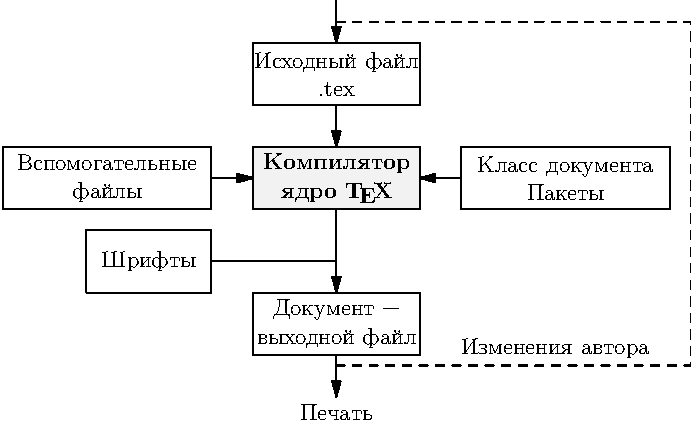
\includegraphics[scale=0.8]{CH-MainFile/Fig-MainFile-1}
\caption{Упрощённая схема работы}
\label{Fig:MainFile-1}
\end{figure}

В процессе работы компилятора в зависимости от задач \TeX\ создаёт \bi{вспомогательные файлы}\index{Файл!вспомогательный}, которые необходимы, например, для хранения данных о ссылках или записи информации о компиляции. Среди них можно выделить следующие основные типы файлов по их расширению:
% % ССЫЛКИ - 4 слова в одном предложении
\begin{description}
\item[\texttt{aux}] отвечает за перекрёстные ссылки и содержит информацию о настройках языка и о тех объектах, на которые можно ссылаться (более подробно см.\ главы~\ref{CH:Sections}, \ref{CH:Itemize}, \ref{CH:Lists}, \ref{Floats});
\item[\texttt{toc}] отвечает за создание оглавления и содержит данные о всех заголовках и страницах, где они начинаются (подробнее см.\ главу~\ref{CH:Sections});
\item[\texttt{lof}, \texttt{lot}] отвечают за списки рисунков и таблиц (см.\ главу~\ref{CH:Floats});
\item[\texttt{log}] содержит информацию о ходе компиляции и возможных предупреждениях и ошибках. Обычно эта информация выводится в специальном окне редактора;
\item[\texttt{idx}, \texttt{ilg}, \texttt{ind}] отвечает за предметные указатели (подробнее в гл.~\ref{CH:Lists});
\item[\texttt{bbl}] появляется при создании списка литературы с помощью Bib\TeX\ (см.\ главу~\ref{CH:BibTeX}).
\end{description}

Исходный файл, в котором происходит вся работа автора, имеет чёткую структуру и состоит из двух основных частей: \emph{преамбулы} и \emph{основного текста}.

\index{Преамбула}\bi{Преамбулой} называется та часть исходного файла, в которой вводятся все необходимые определения и настройки, такие как \emph{класс документа}, \textit{пакеты}, параметры и \textit{макроопределения}. Преамбула основного файла всегда начинается с определения \emph{класса документа}.

\begin{note}
В преамбуле может быть сколько угодно пустых строк, которые никак не влияют на результат.
\end{note}

\index{Текст!основной}\bi{Основной текст} "--- это непосредственно та часть исходного файла, в которой автор набирает всё то, что он хочет видеть в своем документе: текст, таблицы, рисунки и~т.~д. По сути здесь находится весь текст с включёнными в него командами, которые непосредственно влияют на текст, его форматирование и внешний вид.

Таким образом, структуру основного файла можно представить в следующем виде:
\begin{verbatim}
Начало исходного файла
  Преамбула:
   определения и настройки

  Основной текст:
   смысловая часть текста и включённые в неё команды
Конец исходного файла
\end{verbatim}

\begin{note}
Важно отметить, что исходный файл не должен содержать какие бы то ни было выделения цветом, шрифтовые выделения, разбивку на страницы и другие <<художественные>> элементы. Компилятор должен получить <<чистый>> текстовый файл, поэтому наиболее простыми вариантами для набора будут специальные \TeX-редакторы (см.\ параграф~\ref{Sec:Editors}).
\end{note}





% % ========================================================================
\section{Синтаксис и команды языка}\label{Sec:Syntaxis}

Для дальнейшего и более детального изучения строения исходного файла и его содержания рассмотрим вначале особенности синтаксиса\index{Синтаксис языка \TeX} языка системы \TeX\ и языка макроопределений \LaTeX.

% Садовский П.А., 2005/09/18 \bi{Язык системы \TeX}\index{Язык \TeX} и его последующее развитие (например, макропакет \LaTeX\ на основе языка \TeX) не является просто языком разметки, с помощью которого в процессе трансляции документ форматируется определённым образом. Это, можно сказать, полноценный и очень мощный язык программирования, включающий в себя различные средства (например, операторы логических переходов, переопределения команд и~пр.). % Садовский П.А., 2005/09/18

В тексте исходного файла можно использовать латинские и русские буквы \texttt{A}... \texttt{Z}, \texttt{a}... \texttt{z}, \texttt{А}... \texttt{Я}, \texttt{а}... \texttt{я}, цифры \texttt{0}... \texttt{9}, символы:

\begin{verbatim}
. , : ; ! ? ( ) [ ] ' ` - * /  @ | < > + = " №
\end{verbatim}
Кроме того, существует десять зарезервированных символов:
\begin{verbatim}
\ { } $ & # % ^ _ ~
\end{verbatim}
Их употребление в тексте может привести к ошибке или нежелательным последствиям "--- в большинстве случаев, если даже и не будет ошибки, результат вряд ли совпадёт с ожидаемым. Более подробно набор таких символов описан в последующих главах (например, см.\ параграф~\ref{Sec:Znaki}).

\begin{note}
Отметим, что символы <<\verb"|">>, <<\verb|<|>> и <<\verb|>|>> могут встречаться и в командах, но их использование в обычном тексте не приведёт к~ошибке, правда, результат может быть неожиданным.
\end{note}

Команды и макроопределения, составляющие разметочную часть языка \TeX, имеют ряд особенностей и~легко отличаются от обычного текста. %Для их написания используются наиболее редкие для повседневных документов символы.

\bi{Команда}\index{Команда \TeX} "--- это последовательность символов, которая воспринимается транслятором не как обычный текст, а~как указание для совершения какого-либо действия над документом или его частью.

Одной из самых простых команд системы \TeX\ является одиночный символ \verb|%|. Если поставить такой символ в тексте, то все, что идёт после этого символа до перехода на новую строку будет рассматриваться как комментарий и не будет восприниматься компилятором.

Команда системы \TeX{} "--- это либо символы \verb|{|, \verb|}|, \verb|$|, \verb|%|, \verb|&|, либо последовательность символов, которая начинается с <<обратной косой черты>> \verb|\|, например, \verb|\newpage|, \verb|\usepackage[T2A]{fontenc}| и~т.~д., в общем случае имеет вид:
\begin{verbatim}
\<название>[<параметры>]{<параметры>}...{<параметры>}
\end{verbatim}
Заметим, что символ <<\verb|\|>> и \verb|<название команды>| не разделяются пробелом. Окончанием команды является ближайший идущий после неё пробел, переход на новую строку или любой символ, не являющийся командой или буквой латинского алфавита. В квадратных скобках указываются необязательные параметры, а в фигурных "--- обязательные.

В случае, если необязательные \texttt{<параметры>} отсутствуют,  пустые квадратные скобки как ставить, так и опускать их. Например, следующие две команды эквивалентны:
\begin{verbatim}
\<название>[]{<параметры>}
\<название>{<параметры>}
\end{verbatim}

\begin{note}
Во всех описаниях начало и конец строки-названия отмечены открывающей и закрывающей угловыми скобками \verb|<| и \verb|>| соответственно. Они не являются частью команды и введены только для обозначения символьных последовательностей (имён) как единого целого.
\end{note}

Пара символов \verb|{| и \verb|}| используется как ограничители групп текста, которые входят в состав сложных команд или над которым производится некоторое действие. Символ \verb|$| иногда может встречаться в сложных командах, а также (как и символы \verb|_| и \verb|^|) он может использоваться при наборе математических формул.

Отдельно следует выделить команды, которые идут парой и модифицируют текст, заключённый между ними.

\bi{Окружением}\index{Окружение} будем называть <<сдвоенную>> команду системы \LaTeX, выполняющую определённые операции над текстом, заключённым в <<тело окружения>>. Обычно эта команда имеет вид:
\begin{verbatim}
\begin{<имя окружения>}[<параметры>]
  <Тело окружения>
\end{<имя окружения>}
\end{verbatim}

Параметр \verb|<имя окружения>| является обязательным и представляет собой строку "--- название окружения. Дополнительные \texttt{<параметры>} зависят от конкретного окружения и будут каждый раз оговариваться отдельно.

Под \verb|<телом окружения>| будем понимать ту часть текста, к которой применяется данное окружение, т.~е. текст, заключённый между командами начала \verb|\begin{<имя окружения>}| и окончания \verb|\end{<имя окружения>}|.

Окружения в системе \LaTeX\ играют очень важную роль, а их количество и разнообразие очень сильно упрощает работу над текстом и вёрстку документа. Следует отметить, что каждому началу окружения \verb|begin| всегда должен соответствовать свой \verb|end| с тем же самым именем, иначе компилятор выдаст сообщение об ошибке.

\begin{note}
Любая последовательность символов, идущая после \verb|%| до ближайшего перехода на новую строку, рассматривается как комментарий и не воспринимается компилятором.
\end{note}





% % ========================================================================
\section{Простейший вид исходного файла. Первый документ}\label{Sec:FirstDoc}

Как упоминалось ранее, исходный файл, в котором происходит вся работа, состоит из \emph{преамбулы} и \emph{основного текста}. Преамбула всегда начинается с определения класса документа. \bi{Стиль документа}\index{Документ!стиль} или \bi{класс документа}\index{Документ!класс} "--- это тип того документа, который создаёт автор. От выбора этого типа зависят исходные размеры листа и текстовых полей, оформление заголовков, автоматическая нумерация и многие другие настройки.

Класс документа задаётся командой
\begin{verbatim}
\documentclass{<класс документа>}
\end{verbatim}
где обязательный параметр \verb|<класс документа>| представляет собой название того класса, который будет использоваться при создании документа и которому соответствует одноимённый файл
\begin{verbatim}
<класс документа>.cls
\end{verbatim}
При компиляции \TeX\ ищет файл соответствующего класса \verb|*.cls| и берёт из него основные определения и параметры. 

Основной текст, в котором заключена вся смысловая часть документа, набирается в окружении \texttt{document}, т.~е.
\begin{verbatim}
\begin{document}
   <основной текст>
\end{document}
\end{verbatim}

\begin{note}
Любой текст, идущий после строки \texttt{\textbackslash end\{document\}}, не воспринимается \TeX'ом и выводиться не будет.
\end{note}

Таким образом, минимально необходимый для начала работы исходный файл можно представить следующим образом:
\begin{verbatim}
\documentclass{<класс документа>}

\begin{document}
   <основной текст>
\end{document}
\end{verbatim}

Выведем на листе надпись ``This is \TeX!'' с характерным написанием названия \TeX\indcom{TeX}, которое задаётся командой \verb|\TeX|. Эта надпись пока что будет на английском, поскольку этот язык поддерживается по умолчанию.
\begin{example}
This is \TeX!
\end{example}
\begin{release}
\begin{verbatim}
\documentclass{article}

\begin{document}
This is \TeX!
\end{document}
\end{verbatim}
\end{release}

После набора этого текста в \TeX-редакторе и его последующей компиляции в любой из форматов вывода, например, в \verb|pdf|, получаем следующий результат: на листе формата А4 вверху будет нужная нам фраза, а внизу "--- номер страницы.

\begin{remark}
Мы использовали в этом примере один из стандартных классов \texttt{article} (статья), общее описание которого, а также других классов, приводится в параграфе~\ref{Sec:StandardClasses}.
\end{remark}

Сделаем краткие выводы, необходимые для работы.

\begin{enumerate}
\item Исходный файл всегда начинается командой \texttt{\textbackslash documentclass} с указанием класса документа.
\item Основной текст набирается строго внутри окружения \texttt{document}.
\item Любой текст, идущий после строки \texttt{\textbackslash end\{document\}}, не воспринимается \TeX'ом и выводиться не будет.
\item Между определением класса документа и основным  текстом, т.~е.\ в преамбуле, могут идти различные настройки и дополнительные определения.
\end{enumerate}

\begin{note}
Здесь и далее мы будем говорить, что если нужно что-то определить или добавить в преамбулу, это означает, что необходимые строки добавляются \emph{после} определения класса документа и \emph{до} начала окружения \texttt{document}.
\end{note}







% % ========================================================================
\section{Подключение русского языка}\label{Sec:Russian}

В предыдущем примере мы выводили на экран фразу на английском языке. Для использования русского языка нам нужно будет использовать дополнительные \emph{пакеты}.

\bi{Пакет} (или package)\index{Пакет}\index{Package} "--- это набор макрокоманд или макроопределений, расширяющих возможности системы. Эти команды оформлены в виде отдельного одноимённого файла \verb|<пакет>.sty|, где последовательность \verb|<пакет>| "--- имя соответствующего пакета. Более подробно макрокоманды описываются в главе~\ref{CH:Macros}.

Для того чтобы загрузить пакеты с дополнительными макроопределениями для расширения функциональных возможностей системы, используется команда \indcmd{usepackage}, которая имеет вид:
\begin{verbatim}
\usepackage[<опции>]{<пакет>}
\end{verbatim}
Эта команда имеет два параметра. Необязательные \texttt{<опции>} определяют особенности подгружаемого пакета (или пакетов) и могут быть опущены. В этом случае можно как ставить пустые квадратные скобки, так и опускать их. Например, следующие две команды эквивалентны:
\begin{verbatim}
\usepackage[]{<пакет>}
\usepackage{<пакет>}
\end{verbatim}
Параметр \verb|<пакет>| определяет непосредственно сам пакет (точнее, его имя), воплощённый в одноимённом файле под названием \verb|<пакет>.sty|. Заметим также, что эта команда допускает перечисление нескольких пакетов, имена которых указываются через запятые, например,
\begin{verbatim}
\usepackage{<пакет1>,<пакет2>,...,<пакетN>}
\end{verbatim}

\begin{note}
Если были указаны какие-либо параметры, то они передаются \emph{всем} пакетам, указанным в аргументе \comm{usepackage}. Так как этими пакетами могут поддерживаться не все параметры, то следует быть осторожным.
\end{note}

Для использования русского языка необходимо в преамбуле добавить следующие строки
\begin{verbatim}
\usepackage[cp1251]{inputenc}
\usepackage[T2A]{fontenc}
\usepackage[russian]{babel}
\end{verbatim}

Первая команда загружает пакет \texttt{inputenc}, который определяет, какую входную кодировку должен использовать \LaTeX\index{Файл!кодировка}\index{Пакет!inputenc} (см.\ параграф~\ref{CH:Text}).

Вторая команда загружает пакет \texttt{fontenc}, определяющий кодировку шрифта\index{Пакет!fontenc}. В данном случае загружается кодировка \texttt{T2A}, которая используется при русскоязычном наборе. Кодировка шрифта для набора латинского шрифта (английского языка) загружается по умолчанию.

Третья команда загружает пакет, позволяющий использовать и вводить русский язык, корректно расставлять русские переносы\index{Пакет!babel}. Именно поэтому в качестве необязательного параметра указан \texttt{russian}. Для подключения других языков и их переключения в процессе работы "--- см.\ главу~\ref{CH:Fonts}.\medskip

Пусть нам нужно вывести на экран (или последующую печать) следующую строку:
\begin{verbatim}
В любой работе есть место творчеству.
\end{verbatim}

В исходном файле необходимо написать следующее:
\begin{verbatim}
\documentclass{article}
\usepackage[cp1251]{inputenc}
\usepackage[T2A]{fontenc}
\usepackage[russian]{babel}

\begin{document}
В любой работе есть место творчеству.
\end{document}
\end{verbatim}

После компиляции в любой из форматов вывода, на выходе получается следующий результат (при просмотре в программе, соответствующей формату выходного файла): на листе формата А4 внизу будет стоять номер~1, а вверху страницы будет выведена надпись:
\medskip

В любой работе есть место творчеству.

\medskip

Таким образом, приведённый пример уже позволяет работать в системе и набирать тексты на русском языке. Дальнейшие главы будут посвящены тому, как лучше набирать и оформлять тот или иной элемент документа.


\endinput
%Команда {documentclass}\index{Документ!класс}
%\begin{verbatim}
%\documentclass[<параметры класса>]{<класс документа>}
%\end{verbatim}
%имеет два параметра.
%
%Заключённые в квадратные скобки \verb|<параметры класса>| оп\-ределяют размеры листа, шрифта, режима вывода текста и~т.~д. Квадратные скобки указывают на то, что этот параметр является \textit{необязательным}, следовательно, если его опустить (и опустить сами скобки), то все настройки будут ставиться <<по умолчанию>>, например,
%\begin{verbatim}
%\documentclass{<класс документа>}
%\end{verbatim}
%Параметр \verb|<класс документа>|, заключённый в фигурные скобки, является строго обязательным и представляет собой название класса, которому соответствует одноимённый файл
%\begin{verbatim}
%<класс документа>.cls
%\end{verbatim}
%При начале трансляции файл соответствующего класса \verb|*.cls| сначала ищется в текущей папке, в которой лежит исходный файл, а затем, при его отсутствии, в корневых каталогах \TeX'а, указанных в программе <<Mik\TeX{} Options>> на вкладке <<Roots>>, в том порядке, в котором они указаны (обычно это каталоги \texttt{localtexmf} и \texttt{texmf}).

%Поэтому, при создании своих классов или использовании не\-стандартных, соответствующий файл класса с расширением \verb|cls| проще всего, да и лучше, поместить в папку, где находится исходный файл.

%Под определениями и настройками подразумеваются любые настройки документа: поля, шрифты и многое--многое другое. Все они должны находиться после определения класса и до начала основного текста. \bi{Пакет}\index{Пакет}\index{Package} "--- это набор макрокоманд или макроопределений, расширяющих возможности системы и оформленных в виде отдельного <<стилевого>> файла \verb|<пакет>.sty|, где последовательность \verb|<пакет>| "--- имя соответствующего пакета.






